%-------------------------------------------------------------------------
% Design Project Input/Output Module Description
%-------------------------------------------------------------------------

\clearpage
\section{Temperature Input Module}
\label{sec-input-temperature}

This input module enables your IoT device to sense the temperature of
the environment using an easy-to-use temperature sensor. The TMP36
temperature sensor contains an integrated circuit with a simple
interface of three pins: power, signal, and ground. The signal pin's
voltage rises and falls depending on the ambient temperature at
\wu{10}{mV} per degree centigrade (Celsius).

A sample circuit and Arduino code is shown below to get you started.
There is no need for any extra components; we directly connect the
middle pin on the temperature sensor to an analog input on the Arduino.
Make sure the sensor's "flat end" is facing the correct direction (shown
in the diagram). If you point the flat end of the sensor to your left,
then the top pin connects to power (the red wire), the middle pin is the
signal, and the bottom pin connects to ground (the black wire).

The example code will print the analog reading from the temperature
sensor on the serial monitor, similar to how we printed the analog
reading from the grayscale sensor in Lab~2. After setting up the circuit
and programming the Arduino, open the serial monitor and check the
reported room temperature in degrees centigrade. Does the reading sound
right? Experiment with the sensor by changing the ambient temperature
(e.g., using a hair dryer) and see how warm or cool you can make it!

\vspace{0.1in}
\begin{minipage}[t]{0.49\tw}
  \vspace{0pt}

  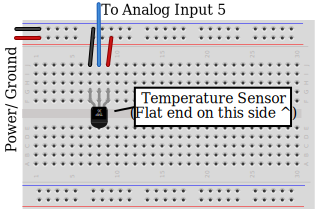
\includegraphics[width=\tw]{input-temperature-annotated.svg.pdf}
\end{minipage}
\hfill
\begin{minipage}[t]{0.49\tw}
  \vspace{0.1in}
  \begin{Verbatim}[gobble=3,fontsize=\small]
    int pin_temperature = 5;

    void setup() {
      Serial.begin(9600);
      pinMode( pin_temperature, INPUT );
    }

    void loop() {
      float temperature = getTemperature( pin_temperature );
      Serial.println( temperature );
      delay(1000);
    }
  \end{Verbatim}
\end{minipage}
\vspace{0.1in}

%Questions:
